%=================================================================
% Template for Drones (MDPI)
%=================================================================
\documentclass[drones,article,submit,pdftex,moreauthors]{Definitions/mdpi}

%=================================================================
% Metadata
%=================================================================
\firstpage{1}
\makeatletter
\setcounter{page}{\@firstpage}
\makeatother
\pubyear{2026}
\articlenumber{0}
\doinum{10.3390/dronesXXXXXX}
\datereceived{XX}
\dateaccepted{XX}
\datepublished{XX}
\copyrightyear{2026}
\externaleditor{XXXXX}

\setlength{\headheight}{20pt}

%=================================================================
% Packages
%=================================================================
\usepackage{amsmath,amssymb,amsfonts}
\usepackage{microtype}
\usepackage{booktabs}
\usepackage{colortbl,xcolor}

%=================================================================
% Title and Authors
%=================================================================
\Title{From Virtual-Point Tracking to an Auditable Geometry-Basis Guidance Interface for Close-Range UAV Interaction}

\Author{Yu Lai$^{1}$,
Yong Chen$^{1}$,
Yang Yang$^{1}$,
Jialong Jian$^{1,}$*,
and Yuanfei Liu$^{1,}$*}

\AuthorNames{Yu Lai, Yong Chen, Yang Yang, Jialong Jian, and Yuanfei Liu}

\address{%
$^{1}$ \quad Aviation Engineering School, Air Force Engineering University, Xi'an 710038, China
}

\corres{Correspondence: j330809@163.com (J.J.); 13572287887@163.com (Y.L.)}

%=================================================================
% Abstract and Keywords
%=================================================================
\abstract{%
Virtual-point guidance provides a compact control interface for autonomous unmanned aerial vehicles, yet conventional Cartesian offset actions do not clearly express the geometry that the controller is attempting to create. This weakens auditability, complicates failure analysis, and obscures why learned behaviour changes across encounter conditions. We reinterpret the unchanged three-dimensional action head as a \emph{geometry-basis guidance interface} whose coefficients modulate longitudinal, lateral, and vertical geometry components. The interface is paired with step-level telemetry and aggregate diagnostics, including a pre-merge Forward Bias metric, $d_{\mathrm{fwd}}$, that links output semantics to trajectory behaviour. Under a 10-seed pilot protocol with a high-fidelity JSBSim flight-dynamics model, we compare the baseline Cartesian policy with broad, narrow, and mixed geometry-basis finetune variants across frontal and crossing encounters against expert and end-to-end learned counterpart controllers. Broad global scaling produces the largest geometry shift but destabilises some cells, most notably reducing frontal expert favourable outcome rate from 0.60 to 0.00. Narrow scaling repairs that lane but introduces regressions elsewhere. The mixed task-selective variant provides the strongest pilot balance: under the expert controller, frontal favourable outcome rate increases to 1.00 while damage margin rises from $13.15$ to $39.65$; crossing favourable outcome rate improves from 0.30 to 0.90 with a positive damage margin of $2.05$. These pilot-scale results support a bounded claim: virtual-point guidance can be recast as an auditable geometry-shaping interface, but stable performance depends on task-conditioned extent design rather than universal amplitude scaling.
}

\keyword{virtual-point guidance; unmanned aerial vehicle; auditable interface; geometry shaping; geometry diagnostics; trustworthy autonomy}

\begin{document}

\section{Introduction}

Autonomous UAV systems are increasingly expected to satisfy performance, safety, and accountability requirements that extend beyond raw task success \cite{elmokadem2021,paterson2025,gunning2019}. In learning-based control pipelines, this raises a practical demand for guidance interfaces that are not only effective in closed-loop operation, but also interpretable enough to support trust, failure diagnosis, and certification-oriented assessment \cite{glanois2024,paterson2025,thomas2021}. Virtual-point guidance remains attractive in this setting because it provides a compact mechanism for steering motion through point-relative commands and can be integrated naturally with modern policy learners \cite{zarchan2012}. However, when the policy output is exposed only as Cartesian virtual-point offsets, the action layer communicates little about the geometry that the controller is attempting to create \cite{lai2026aerospace}. As a result, the interface can remain operationally useful while still being difficult to audit when behaviour changes across close-range encounter conditions.

This paper addresses that gap by reinterpreting the existing three-dimensional virtual-point action head as an auditable geometry-basis guidance interface \cite{xu2022ast}. Rather than introducing a new policy architecture, we preserve the network structure and action dimensionality and instead reconstruct the semantics of the output layer so that the three coefficients correspond to longitudinal, lateral, and vertical geometry components. We pair this interface with step-level telemetry and aggregate geometry diagnostics, including a pre-merge Forward Bias metric, $d_{\mathrm{fwd}}$, to expose how action semantics are translated into trajectory-level behaviour \cite{lai2026aerospace}. Using this formulation, we compare baseline, broad, narrow, and mixed interface variants across frontal and crossing close-range UAV interactions under expert-controller and end-to-end learned-controller settings. Our goal is not to claim that a universally best policy has been found, but to show that geometry shaping can be made auditable and that stable behaviour depends on task-conditioned interface design rather than uniform global scaling \cite{wang2023aerospace}.

This motivation sits at the intersection of three established research threads. First, virtual-target and look-ahead guidance methods have long shown that carefully chosen geometric reference points can improve path-following performance, curved-trajectory convergence, and anticipatory behaviour in UAV guidance \cite{park2007,ratnoo2015,breivik2005}. Second, reinforcement learning has become an increasingly common tool for autonomous UAV control and manoeuvre generation, ranging from modular flight-control decomposition to direct decision policies in dynamic interaction settings \cite{choi2023,quan2026,wang2023aerospace}. Third, interpretability and assurance research has argued that high-stakes autonomy cannot be justified by aggregate performance alone; it also requires inspectable representations, traceable evidence, and interfaces that expose the basis of decision making \cite{glanois2024,paterson2025,paleja2022}. What remains underexplored is how these threads can be combined at the guidance interface layer itself.

Accordingly, this study makes three bounded contributions. First, it reformulates the existing three-dimensional virtual-point action head as a geometry-basis interface without changing the policy network or the downstream guidance stack. Second, it introduces an audit trail consisting of step-level telemetry, separated termination semantics, and the pre-merge Forward Bias diagnostic. Third, it uses a controlled pilot comparison of baseline, broad, narrow, and mixed variants to show that stable geometry shaping is task-conditioned rather than well served by universal amplitude scaling. The remainder of the paper is organised as follows. Section~2 reviews prior work on virtual-target guidance, learning-based UAV control, and interpretable autonomy. Section~3 introduces the geometry-basis interface and its diagnostic instrumentation. Section~4 describes the experimental protocol, Section~5 reports the comparative results, and Section~6 discusses implications. Section~7 notes limitations and responsible use, and Section~8 concludes the paper.

\section{Related Work}

\paragraph{Virtual-target and path-following guidance.}
Reference-point guidance has a long history in autonomous vehicle navigation, especially in settings where the controlled vehicle must converge smoothly to a path or moving spatial objective rather than simply minimise instantaneous position error \cite{sujit2014}. Park, Deyst, and How formalised a nonlinear path-following guidance method that uses a forward reference point to generate anticipatory lateral acceleration and improve curved-trajectory tracking \cite{park2007}. Ratnoo et al.\ later showed that trajectory-shaping guidance can be interpreted through a virtual-target perspective and can reduce the limitations associated with naive pure-pursuit behaviour \cite{ratnoo2015}. In the broader UAV literature, these virtual-target ideas remain attractive because they provide geometric intuition, low online complexity, and a clean separation between outer-loop guidance and inner-loop stabilisation \cite{elmokadem2021,rhee2010}. Our work inherits that geometric-guidance lineage, but shifts the design question from how to place a virtual point along a predefined path to how a learned policy should semantically parameterise the geometry of that point.

\paragraph{Learning-based UAV control and decision policies.}
Recent UAV autonomy research has increasingly used reinforcement learning to replace or augment hand-crafted logic in tracking, flight control, and sequential decision making. Choi et al.\ proposed a modular reinforcement-learning architecture for autonomous UAV flight control, emphasising decomposition and policy reuse across subtasks rather than a monolithic end-to-end controller \cite{choi2023,jing2024aerospace}. More recently, Quan et al.\ used a soft actor--critic framework for autonomous UAV manoeuvre decision making, reflecting the broader shift toward directly learned policies for rapidly changing interaction settings \cite{quan2026,haarnoja2018}. These studies illustrate the practical momentum behind learned UAV guidance, but they also reflect a common pattern: the emphasis is usually placed on policy learning strategy, algorithm choice, or modular decomposition, while the semantic transparency of the output interface remains secondary. In contrast, the present study keeps the policy network fixed and focuses on making the action interface itself more interpretable and more diagnosable.

\paragraph{Interpretable reinforcement learning and trustworthy autonomy.}
Interpretability research in reinforcement learning has highlighted the distinction between post-hoc explanations and policies whose internal representations or decision variables are directly inspectable \cite{glanois2024,paleja2022}. For autonomous systems, this distinction matters because deployment confidence depends not only on predictive accuracy or reward optimisation, but also on whether the evidence needed for verification, diagnosis, and assurance can be systematically assembled \cite{paterson2025,gunning2019}. In UAV systems specifically, the push toward greater autonomy has amplified the need for trustworthy interfaces that expose why a controller behaves differently across environments and operating conditions \cite{elmokadem2021,thomas2021}. Our work addresses this need at a different layer than most explainable-RL approaches: instead of explaining a trained policy after the fact or redesigning the full learning architecture, we reconstruct the semantics of the existing output space into a white-box geometry-basis layer with explicit telemetry and aggregate diagnostics. This makes the learned controller easier to audit while preserving the original network and action dimensionality.

\section{Materials and Methods}

\subsection{Overview}

Our study compares four guidance-interface variants under a common high-fidelity flight-dynamics model (JSBSim) \cite{lai2026aerospace}. All variants share the same policy network, observation schema, reward definition, and downstream guidance stack. The only differences lie in the action-to-virtual-point mapping and the associated diagnostic instrumentation. The four compared methods are: (1)~a \emph{baseline} using Cartesian virtual-point semantics; (2)~a \emph{broad} geometry-basis finetune with large, unselective extents; (3)~a \emph{narrow} geometry-basis finetune with substantially reduced extents; and (4)~a \emph{mixed} task-selective geometry-basis finetune that preserves narrow frontal extents while restoring crossing extents. Section~3.1 presents the baseline formulation; Section~3.2 introduces the geometry-basis action semantics; Section~3.3 defines the Forward Bias metric; and Section~3.4 describes the telemetry and aggregate diagnostics pipeline.

\subsection{Baseline Virtual-Point Guidance Formulation}

Let $\mathbf{p}^{\mathrm{anc}}_t \in \mathbb{R}^3$ denote the anchor position selected at time step $t$ by the existing virtual-point guidance stack \cite{xu2022ast}. Within the present study scope, the learned policy outputs a three-dimensional action vector
\begin{equation}
\mathbf{u}_t = [u_x, u_y, u_z]^\top \in [-1,1]^3.
\end{equation}
Under the baseline Cartesian semantics, this action is mapped to a frame-dependent displacement,
\begin{equation}
\Delta \mathbf{p}^{\mathrm{cart}}_t =
\mathcal{T}_f
\left(
\begin{bmatrix}
S_x u_x \\
S_y u_y \\
S_z u_z
\end{bmatrix}
\right),
\end{equation}
where $S_x$, $S_y$, and $S_z$ are axis scales in metres and $\mathcal{T}_f(\cdot)$ maps the configured local offset frame $f$ into world coordinates. The resulting virtual point is then
\begin{equation}
\mathbf{p}^{\mathrm{vp}}_t = \mathbf{p}^{\mathrm{anc}}_t + \Delta \mathbf{p}^{\mathrm{cart}}_t.
\end{equation}
All other components of the guidance pipeline are preserved: anchor selection, predicted-reference blending, close-range anchor rewrites, release and recovery logic, and the downstream line-of-sight tracking layer. This baseline formulation therefore provides a controlled reference in which the output semantics can be modified without changing the policy backbone or the downstream guidance stack.

\subsection{Geometry-Basis Action Semantics}

\textbf{Motivation.} The baseline Cartesian formulation treats the three action dimensions as independent world-axis offsets. This representation is compact, but it has a practical limitation: the policy output does not carry explicit geometric meaning. A positive $u_x$ may correspond to a lead placement in one encounter geometry and a lag placement in another, depending on the active frame transform. This opacity makes it difficult to diagnose whether a given trajectory shape is an intended behaviour or an artefact of frame coupling, and it complicates the comparison of learned policies across different interface configurations \cite{lai2026aerospace}. To address this, we seek a representation in which the action coefficients directly encode longitudinal, lateral, and vertical geometry decisions with respect to the encounter geometry.

\textbf{Design.} The proposed interface preserves the same three-dimensional action head but changes its interpretation. Instead of reading $\mathbf{u}_t$ as Cartesian offsets, we interpret it as geometry-basis coefficients
\begin{equation}
\mathbf{a}_t = [a_{\mathrm{ll}}, a_{\mathrm{io}}, a_{\mathrm{cd}}]^\top \in [-1,1]^3,
\end{equation}
corresponding to lead--lag, inside--outside, and climb--descent components, respectively. The world-coordinate virtual-point displacement becomes
\begin{equation}
\Delta \mathbf{p}^{\mathrm{gb}}_t
=
a_{\mathrm{ll}} \mathbf{b}_{\mathrm{ll},t}
+ a_{\mathrm{io}} \mathbf{b}_{\mathrm{io},t}
+ a_{\mathrm{cd}} \mathbf{b}_{\mathrm{cd},t},
\label{eq:geometry_basis_offset}
\end{equation}
where $\mathbf{b}_{\mathrm{ll},t}$, $\mathbf{b}_{\mathrm{io},t}$, and $\mathbf{b}_{\mathrm{cd},t}$ are the basis vectors expressed in world coordinates. These vectors are constructed from fixed-magnitude template offsets and transformed through task-relevant frames:
\begin{align}
\mathbf{b}_{\mathrm{ll},t} &= \mathcal{T}_{\mathrm{long}}
\left(
\begin{bmatrix}
L_{\mathrm{ll}} \\
0 \\
0
\end{bmatrix}
\right), \\
\mathbf{b}_{\mathrm{io},t} &= \mathcal{T}_{\mathrm{lat}}
\left(
\begin{bmatrix}
0 \\
s_{\mathrm{lat}} L_{\mathrm{io}} \\
0
\end{bmatrix}
\right), \\
\mathbf{b}_{\mathrm{cd},t} &= \mathcal{T}_{\mathrm{vert}}
\left(
\begin{bmatrix}
0 \\
0 \\
L_{\mathrm{cd}}
\end{bmatrix}
\right).
\end{align}
Here, $L_{\mathrm{ll}}$, $L_{\mathrm{io}}$, and $L_{\mathrm{cd}}$ are extent parameters in metres, while $s_{\mathrm{lat}} \in \{-1, +1\}$ keeps the lateral basis orientation consistent across mirrored encounter geometries. In the implementation used here, the longitudinal basis is aligned with the target-velocity frame, the lateral basis uses an encounter-stable frame, and the vertical basis is aligned with the world NEU frame. Positive coefficients correspond to lead, outside, and climb tendencies; negative coefficients correspond to lag, inside, and descent tendencies. The virtual point is then
\begin{equation}
\mathbf{p}^{\mathrm{vp}}_t = \mathbf{p}^{\mathrm{anc}}_t + \Delta \mathbf{p}^{\mathrm{gb}}_t.
\end{equation}
Because the anchor stack and action dimensionality remain unchanged, the comparison between Cartesian and geometry-basis semantics isolates the effect of output interpretation rather than policy capacity \cite{xu2022ast}.

\textbf{Technical advantage.} The geometry-basis formulation provides three advantages over the Cartesian baseline. First, the coefficient values are directly comparable across encounter geometries because they encode the same semantic direction (lead, outside, climb) regardless of the active frame transform. Second, the extent parameters $L_{(\cdot)}$ provide a compact, interpretable design space for reshaping the realised geometry without retraining the policy. Third, the basis-vector decomposition makes it possible to instrument the interface with per-component telemetry, enabling the diagnostic tools described in Section~3.4 \cite{lai2026aerospace}. Figure~\ref{fig:geometry_basis_interface} summarises the resulting architectural boundary: the policy backbone and three-dimensional action head remain unchanged, while the new semantics layer and its diagnostics become directly auditable.

\begin{figure}[H]
\centering
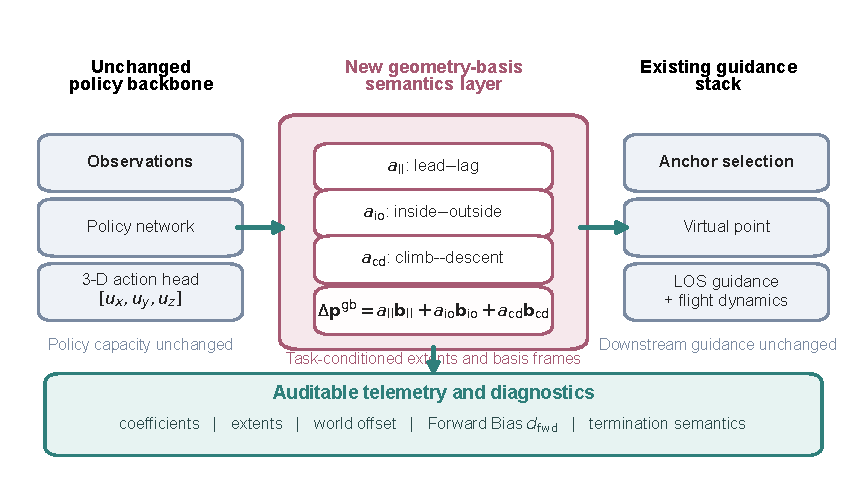
\includegraphics[width=\linewidth]{figures/figure1_geometry_basis_interface.pdf}
\caption{Geometry-basis guidance interface. The policy backbone and three-dimensional action head remain unchanged. The new layer reinterprets the three outputs as lead--lag, inside--outside, and climb--descent coefficients, converts them through task-conditioned basis extents and basis frames, and exposes step-level telemetry and diagnostics including pre-merge Forward Bias and termination semantics.}
\label{fig:geometry_basis_interface}
\end{figure}

\subsection{Forward Bias Definition}

To quantify how strongly the virtual point is placed ahead of or behind the interacting vehicle, we express the relative virtual-point displacement in the target-velocity frame:
\begin{equation}
\mathbf{r}^{\mathrm{tv}}_t
=
\mathcal{T}_{\mathrm{tv}}^{-1}
\left(
\mathbf{p}^{\mathrm{vp}}_t - \mathbf{p}^{\mathrm{tar}}_t
\right)
=
\begin{bmatrix}
d_{\mathrm{fwd},t} \\
d_{\mathrm{lat},t} \\
d_{\mathrm{vert},t}
\end{bmatrix},
\label{eq:forward_bias_vector}
\end{equation}
where $\mathbf{p}^{\mathrm{tar}}_t$ is the target position at time step $t$. The first component, $d_{\mathrm{fwd},t}$, is the instantaneous \emph{Forward Bias}. Positive values indicate that the virtual point lies ahead along the target-velocity direction, whereas negative values indicate a lagging placement behind that direction. For pre-merge analysis, we compute the mean Forward Bias over the set of pre-merge steps $\mathcal{P}$:
\begin{equation}
\bar{d}_{\mathrm{fwd}}^{\mathrm{pre}}
=
\frac{1}{|\mathcal{P}|}
\sum_{t \in \mathcal{P}} d_{\mathrm{fwd},t}.
\label{eq:premerge_forward_bias}
\end{equation}
We use $\bar{d}_{\mathrm{fwd}}^{\mathrm{pre}}$ as the primary geometry-health indicator in the present study because it measures forward placement directly in a physically meaningful frame, remains comparable across all interface variants, and can be computed from the same step-level artefacts used for outcome analysis.

\subsection{Telemetry and Geometry Diagnostics}

The geometry-basis interface is instrumented so that action semantics can be examined at the same temporal resolution as the simulated trajectory. At each step, we record the active action semantics, the coefficient values $(a_{\mathrm{ll}}, a_{\mathrm{io}}, a_{\mathrm{cd}})$, the basis extents $(L_{\mathrm{ll}}, L_{\mathrm{io}}, L_{\mathrm{cd}})$, the world-coordinate basis vectors $\mathbf{b}_{\mathrm{ll},t}$, $\mathbf{b}_{\mathrm{io},t}$, and $\mathbf{b}_{\mathrm{cd},t}$, the composed world offset $\Delta \mathbf{p}^{\mathrm{gb}}_t$, the anchor position, the virtual-point position, and geometry-bias variables including $d_{\mathrm{fwd},t}$ and $d_{\mathrm{lat},t}$. We also retain termination-state markers and unchanged downstream geometry fields so that interface semantics can be interpreted jointly with trajectory outcome.

Aggregate diagnostics are computed by partitioning each trajectory into pre-merge and post-merge segments. For the pre-merge segment, we report $\bar{d}_{\mathrm{fwd}}^{\mathrm{pre}}$ from \eqref{eq:premerge_forward_bias}, the mean geometry-basis coefficients,
\begin{equation}
\bar{a}_{k}^{\mathrm{pre}}
=
\frac{1}{|\mathcal{P}|}
\sum_{t \in \mathcal{P}} a_{k,t},
\qquad
k \in \{\mathrm{ll}, \mathrm{io}, \mathrm{cd}\},
\end{equation}
and the fraction of pre-merge steps with positive lateral coefficient,
\begin{equation}
\phi_{\mathrm{io}}^{+,\mathrm{pre}}
=
\frac{1}{|\mathcal{P}|}
\sum_{t \in \mathcal{P}} \mathbb{I}\!\left(a_{\mathrm{io},t} > 0\right).
\end{equation}
For the post-merge segment, we compute corresponding coefficient means while retaining the existing bias and outcome summaries. The resulting telemetry and diagnostics make it possible to connect output semantics, trajectory geometry, and termination behaviour without relying on outcome rate alone.

\section{Experimental Setup}

\subsection{Simulation Platform and Compared Variants}

All experiments in the present paper were conducted with the JSBSim backend so that the compared policies were evaluated under a common high-fidelity flight-dynamics model. The main comparison anchor was the established baseline virtual-point policy associated with the internal artefact identifier \texttt{reset075\_no\_mode\_switch\_longscale00}. Relative to this baseline, we evaluated three geometry-basis finetune variants while preserving the observation schema, reward definition, action dimensionality, and downstream guidance stack.

The four compared methods were as follows. The \emph{baseline} uses the original Cartesian virtual-point semantics. The \emph{broad} geometry-basis finetune applies an unselective set of relatively large basis extents across both encounter classes, namely $(1200,1600,600)$~m for the frontal encounter and $(800,300,300)$~m for the crossing encounter. The \emph{narrow} variant reduces those extents substantially, yielding frontal-encounter extents of $(L_{\mathrm{ll}},L_{\mathrm{io}},L_{\mathrm{cd}})=(300,600,100)$~m and crossing-encounter extents of $(250,300,75)$~m. The \emph{mixed} task-selective variant retains the narrow frontal-encounter setting while restoring the crossing-encounter extents to $(800,300,300)$~m. All three geometry-basis variants were warm-started from the same baseline checkpoint, so the resulting comparison isolates the effect of interface semantics and extent design rather than changes in policy capacity. Table~\ref{tab:extent_design} summarises the extent parameters for each variant.

\begin{table}[t]
\centering
\caption{Basis extent parameters (metres) for each interface variant. Frontal and crossing encounters use different extent sets because the encounter geometry demands different operating ranges.}
\label{tab:extent_design}
\begin{tabular}{@{}lcccccc@{}}
\toprule
& \multicolumn{3}{c}{Frontal encounter} & \multicolumn{3}{c}{Crossing encounter} \\
\cmidrule(lr){2-4}\cmidrule(lr){5-7}
Variant & $L_{\mathrm{ll}}$ & $L_{\mathrm{io}}$ & $L_{\mathrm{cd}}$ & $L_{\mathrm{ll}}$ & $L_{\mathrm{io}}$ & $L_{\mathrm{cd}}$ \\
\midrule
Baseline & \multicolumn{6}{c}{Cartesian offsets (no geometry-basis extents)} \\
Broad & 1200 & 1600 & 600 & 800 & 300 & 300 \\
Narrow & 300 & 600 & 100 & 250 & 300 & 75 \\
Mixed & 300 & 600 & 100 & 800 & 300 & 300 \\
\bottomrule
\end{tabular}
\end{table}

\subsection{Encounter Classes}

The evaluation scope was intentionally limited to two close-range interaction classes. The first was a \emph{frontal encounter}, in which the two vehicles approached each other in an initially opposing geometry. The second was a \emph{crossing encounter}, in which the counterpart vehicle entered from a lateral crossing geometry. These two classes were chosen because they provide distinct geometry-shaping demands while remaining compact enough for controlled comparative analysis. No additional encounter families were promoted into the main paper narrative.

For the crossing encounter, the close-range admissibility gate used a fixed angle-of-arrival threshold of $60^\circ$ in every run. This setting was held constant for the baseline and all geometry-basis variants so that changes in aggregate behaviour could not be attributed to a looser or tighter entry condition. The crossing-encounter comparison therefore isolates interface effects under a shared close-range gate rather than modifying the geometry envelope itself.

\subsection{Counterpart Controller Split}

To test whether geometry-basis interface changes behave consistently against different interactive behaviours, each method was evaluated against two counterpart-controller classes. The first was an \emph{expert controller}, representing a structured rule-based or expert-designed policy. The second was an \emph{end-to-end learned controller}, representing a fully learned counterpart policy with a different behavioural profile. This split is important because the same geometry-basis modification can appear beneficial under one controller class while degrading behaviour under another. Accordingly, all main results are reported separately for the expert-controller and end-to-end learned-controller settings rather than pooled across them.

\subsection{Pilot Protocol}

The study was conducted as a pilot-scale comparative evaluation rather than a large held-out benchmark. Each method was run with the same 10 evaluation seeds, namely 480 through 489, under a formal-small protocol. This paired-seed design was used for both encounter classes and both counterpart-controller settings, yielding a compact but reproducible comparison grid. We intentionally did not launch a larger formal held-out campaign at this stage, because the paper objective is to characterise auditable interface behaviour and task-conditioned trade-offs rather than to claim a finalised universally stable policy.

Within each cell of the comparison grid, the policy was evaluated under the same backend, initial-health setting, damage-per-step setting, and close-range gate parameters. The mixed, narrow, and broad geometry-basis variants therefore differ from the baseline primarily through the semantics of the action-to-virtual-point mapping and the task-dependent extent parameters used in that mapping.

To keep the comparison traceable, every reported result was derived from preserved seed-level episode records, raw termination reasons, and aggregate geometry diagnostics generated under the same evaluation pipeline. The geometry-basis variants were enabled through configuration changes only; the three-dimensional action head, observation schema, reward definition, and backend were held fixed across the comparison.

\subsection{Evaluation Metrics}

We report five primary metrics together with raw termination semantics. First, we measure the \emph{favourable outcome rate}, denoted here by $r_{\mathrm{fav}}$, which corresponds to the existing evaluator field \texttt{win\_rate} in the reproducibility artefacts:
\begin{equation}
r_{\mathrm{fav}}
=
\frac{1}{N}
\sum_{i=1}^{N}
\mathbb{I}(y_i = \text{favourable}),
\end{equation}
where $y_i$ is the resolved episode outcome for episode $i$. Second, we report the \emph{damage margin},
\begin{equation}
m_{\mathrm{dmg}}
=
\frac{1}{N}
\sum_{i=1}^{N}
\left(
D^{\mathrm{deal}}_i - D^{\mathrm{take}}_i
\right),
\end{equation}
which summarises the mean difference between damage dealt to the counterpart vehicle and damage received by the controlled UAV.

Third, we report \emph{ego crashes}, i.e., the number of episodes in which the controlled UAV terminated through a crash or an out-of-bounds event. Fourth, we report \emph{counterpart crash/out-of-bounds events}, i.e., the number of episodes in which the counterpart vehicle terminated through the same failure modes. These two counts are reported separately because the aggregate artefact field \texttt{crashes} combines them and is therefore insufficient for interpreting which side failed. Fifth, we report the pre-merge Forward Bias $\bar{d}_{\mathrm{fwd}}^{\mathrm{pre}}$ from \eqref{eq:premerge_forward_bias} as the main geometry-health indicator.

In addition to these scalar summaries, we inspect the raw distribution of termination categories for each method--encounter--controller cell. This includes favourable timeout outcomes, unfavourable timeout outcomes, ego crash or out-of-bounds events, and counterpart crash or out-of-bounds events. Termination-category analysis is treated as a first-class result rather than a debugging aid, because it distinguishes geometry-shaping improvements from apparent gains that arise mainly from counterpart failure modes.

\section{Results}

\subsection{Broad Geometry-Basis Finetune}

The broad geometry-basis finetune produced the clearest initial evidence that output semantics can strongly reshape interaction geometry, but it did so in a globally over-amplified manner. Under the expert-controller setting, the frontal-encounter favourable outcome rate collapsed from $0.60$ to $0.00$, while the mean damage margin fell from $13.15$ to $-15.40$~(Table~\ref{tab:main_results}). At the same time, the pre-merge Forward Bias increased from $10.84$~m to $503.65$~m. This is a large geometry shift rather than a marginal parameter effect. By contrast, the crossing encounter under the same controller improved in favourable outcome rate from $0.30$ to $0.90$, but the damage margin still deteriorated from $-0.80$ to $-3.85$, indicating that a higher outcome rate alone did not correspond to cleaner geometry or healthier exchange behaviour.

The end-to-end learned-controller setting showed a different pattern. The frontal encounter remained approximately stable in favourable outcome rate ($0.90 \rightarrow 0.90$) with a small damage-margin increase ($7.30 \rightarrow 9.15$), and the crossing encounter also remained stable in favourable outcome rate ($1.00 \rightarrow 1.00$) with a modest margin increase ($0.75 \rightarrow 2.50$). However, the geometry diagnostics reveal that this apparent stability coincided with a strong positive shift in pre-merge Forward Bias in every lane: $11.94 \rightarrow 498.76$~m for the end-to-end frontal encounter and $-660.51 \rightarrow 183.58$~m for the end-to-end crossing encounter. The same broad variant therefore moved all four cells toward a much more forward-biased geometry, even when the aggregate outcome rate did not immediately collapse.

Raw termination semantics further clarify why the broad variant cannot be treated as a generally successful result. In the expert-controller crossing encounter, the high favourable outcome rate was driven mainly by counterpart crash or out-of-bounds events rather than by cleaner damage-margin improvement. In other words, the broad variant demonstrated that geometry-basis semantics can strongly alter behaviour, but it also showed that unselective global scaling pushes the interface toward an unstable forward-insertion regime. Taken together, these results verify that auditable geometry shaping is real while identifying broad global scaling as too blunt to support a stability claim.

\subsection{Narrow Geometry-Basis Finetune}

The narrow geometry-basis variant partially repaired the instability introduced by the broad setting, but the repair proved to be highly task-dependent. Its clearest success appeared in the frontal encounter under the expert-controller setting. Relative to the broad variant, the pre-merge Forward Bias was reduced from $503.65$~m to $185.92$~m, the favourable outcome rate recovered from $0.00$ to $0.90$, the damage margin increased from $-15.40$ to $23.70$, and the controlled-UAV crash count dropped from 4 episodes to 0. This confirms that shrinking the basis extents can meaningfully reduce overreach when the geometry has become too aggressively forward-biased.

That repair, however, did not generalise across the comparison grid. In the frontal encounter under the end-to-end learned-controller setting, the favourable outcome rate dropped sharply from $0.90$ to $0.20$, while the controlled-UAV crash count increased from 1 to 7 episodes and the damage margin weakened from $7.30$ to $2.25$. A second regression appeared in the expert-controller crossing encounter, where the favourable outcome rate decreased from $0.30$ to $0.20$ and the damage margin worsened from $-0.80$ to $-6.20$. The termination distribution in that cell was dominated by unfavourable timeout outcomes rather than by a clean geometry-driven repair.

The geometry diagnostics show why this result is important. Narrowing the extents reduced pre-merge Forward Bias in all four cells relative to the broad variant, but it did not eliminate the tendency toward positive lead and climb preferences. Instead, it changed the realised geometry mostly by shrinking the metric amplitude of those preferences. The result is therefore not a contradiction of the broad-variant finding; rather, it shows that uniform shrinkage can repair one cell while breaking another. The narrow variant therefore acts less as a final setting than as evidence that globally conservative scaling remains too coarse once encounter class and counterpart behaviour diverge.

\subsection{Mixed Task-Selective Geometry-Basis Finetune}

The mixed geometry-basis variant provided the strongest observed overall balance among the compared methods in the present pilot and is therefore the current main-table candidate. Its design preserved the narrow frontal-encounter extents that repaired the expert-controller frontal case while restoring the crossing-encounter extents to recover lost reach. Under the expert-controller setting, this produced a favourable outcome rate of $1.00$ in the frontal encounter, up from the baseline value of $0.60$, while the damage margin increased from $13.15$ to $39.65$ and the controlled-UAV crash count fell from 2 to 0. In the expert-controller crossing encounter, the favourable outcome rate increased from $0.30$ to $0.90$ and the damage margin improved from $-0.80$ to $2.05$, with no controlled-UAV crashes.

Equally important, the mixed variant avoided the most serious regressions of the narrow setting. In the frontal encounter under the end-to-end learned-controller setting, the favourable outcome rate remained at $0.90$, matching the baseline, while the damage margin improved from $7.30$ to $8.70$ and the controlled-UAV crash count remained at 1 episode. In the end-to-end crossing encounter, the favourable outcome rate stayed at $1.00$, the damage margin increased from $0.75$ to $2.90$, and no controlled-UAV crashes were observed. The mixed variant therefore restored the narrow variant's failure mode in the end-to-end frontal cell without giving back the frontal repair achieved under the expert-controller setting.

Termination-category evidence strengthens this interpretation. In the expert-controller crossing encounter, the mixed variant produced nine favourable timeout outcomes and only one unfavourable timeout outcome, rather than relying mainly on counterpart crash or out-of-bounds events. This distinguishes the mixed variant from the broad variant, whose apparent gain in that cell was largely failure-mode driven. At the same time, the geometry diagnostics show that the mixed variant still maintained positive pre-merge Forward Bias in every cell: $192.51$~m and $234.84$~m under the expert controller, and $173.11$~m and $198.20$~m under the end-to-end learned controller. The implication is not that Forward Bias has become irrelevant; rather, it is that task-selective extent design can channel a forward-biased geometry into a more stable and interpretable operating regime. In the present pilot, the mixed variant therefore provides the strongest empirical support for framing the paper as an auditable interface-design study rather than as a claim of universal policy optimality.

\subsection{Why Outcome Rate Alone Is Insufficient}

The preceding comparisons show that favourable outcome rate is necessary but not sufficient for interpreting interface quality. The clearest example is the crossing encounter under the expert-controller setting for the broad variant. There, the favourable outcome rate rose from $0.30$ to $0.90$, which could easily be misread as a substantial guidance improvement. However, the damage margin simultaneously decreased from $-0.80$ to $-3.85$, and the raw termination records show that the apparent gain was driven primarily by counterpart crash or out-of-bounds events rather than by a cleaner exchange process. In that cell, a high outcome rate did not mean healthier geometry; it mostly meant that the counterpart vehicle failed first.

This example is also where the aggregate artefact field \texttt{crashes} becomes most misleading if read without decomposition. For the broad expert-controller crossing cell, that field would report nine crash-related terminations, but those episodes were composed of zero ego crashes and nine counterpart crash or out-of-bounds events. If the outcome summary and the aggregate crash count were read in isolation, the result could be mistaken for a simultaneously aggressive and successful policy. The episode-level semantics show a different story: the favourable outcome rate was inflated by counterpart failure modes, not by a consistently healthy interaction geometry.

The mixed variant provides an instructive contrast. In the same expert-controller crossing encounter, it also achieved a favourable outcome rate of $0.90$, but the termination categories shifted to nine favourable timeout outcomes and only one unfavourable timeout outcome, while the damage margin became positive at $2.05$. These two cells therefore share the same scalar outcome rate but correspond to materially different interaction structures. The broad variant reached the same headline number through failure-mode dominance, whereas the mixed variant reached it through a more balanced geometry and damage exchange profile.

A paired representative seed in Figure~\ref{fig:representative_case} makes this distinction visible at trajectory level. Under the broad variant, the recorded favourable outcome occurs only because the counterpart leaves the admissible region even though the damage margin is negative. Under the mixed variant, the same initial seed produces a longer bounded interaction that finishes with a favourable timeout and a positive damage margin. The point of the comparison is not that one single seed proves the aggregate result, but that the episode-level geometry is consistent with the termination-category interpretation.

This distinction also appears in the end-to-end learned-controller crossing encounter. Both the baseline and mixed variants achieved a favourable outcome rate of $1.00$, yet the baseline did so entirely through counterpart crash or out-of-bounds events, whereas the mixed variant introduced one favourable timeout outcome and improved the damage margin from $0.75$ to $2.90$. Even when the outcome rate is unchanged, the underlying interaction can become more favourable, more stable, or more interpretable. Figure~\ref{fig:termination_semantics} visualises these termination-category compositions across the full comparison grid. For this reason, all main conclusions in this study are based on the joint reading of favourable outcome rate, damage margin, separated crash counts, and termination-category distributions rather than on a single scalar success summary.

\begin{figure}[H]
\centering
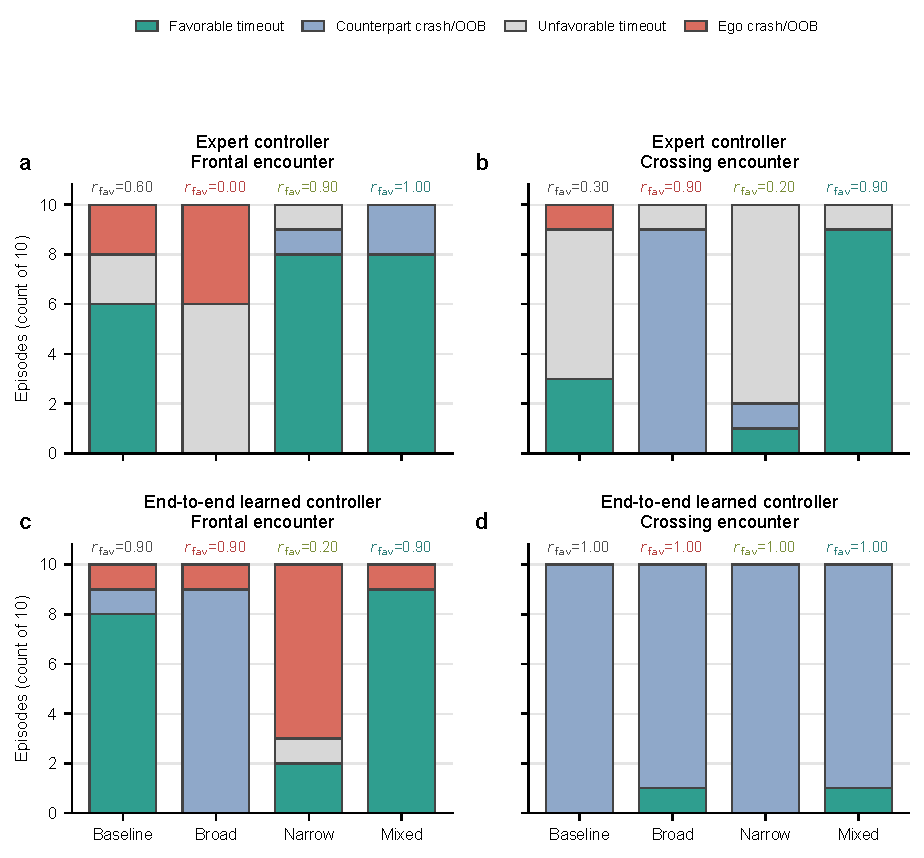
\includegraphics[width=\linewidth]{figures/figure2_termination_semantics.pdf}
\caption{Termination semantics across interface variants. Each stacked bar summarises the 10 pilot episodes for one interface variant. Similar favourable outcome rates can arise from substantially different underlying semantics. In the expert crossing encounter, the broad result is dominated by counterpart crash or out-of-bounds events, whereas the mixed result is dominated by favourable timeout outcomes.}
\label{fig:termination_semantics}
\end{figure}

\subsection{Geometry-Health Interpretation}

Forward Bias provides the clearest aggregate view of how the interface variants reshape geometry across the comparison grid. In the baseline, the frontal encounter began with only a small positive Forward Bias ($10.84$~m under the expert controller and $11.94$~m under the end-to-end learned controller), whereas the crossing encounter began with strongly negative values ($-598.92$~m and $-660.51$~m, respectively). The broad geometry-basis finetune shifted all four cells sharply into the positive range, reaching $503.65$~m, $220.69$~m, $498.76$~m, and $183.58$~m. This confirms that the semantics reinterpretation is not merely cosmetic: it changes the realised geometry in a large and measurable way.

The link between Forward Bias and the main success or failure cases is most visible in the frontal encounters. Under the expert controller, the broad variant combined a very large Forward Bias of $503.65$~m with complete outcome collapse, whereas the narrow and mixed variants reduced that value to $185.92$~m and $192.51$~m and simultaneously removed ego crashes while restoring favourable outcome rates. This is the clearest case in the paper where a reduction in $\bar{d}_{\mathrm{fwd}}^{\mathrm{pre}}$ coincides with a direct repair in geometry health.

The narrow and mixed variants also show why Forward Bias should be treated as a health signal rather than as a one-number explanation. In the end-to-end frontal encounter, the narrow and mixed variants produced very similar Forward Bias values ($169.34$~m and $173.11$~m), yet their termination profiles were very different: the narrow variant produced seven ego crashes and a favourable outcome rate of $0.20$, whereas the mixed variant returned to one ego crash and a favourable outcome rate of $0.90$. Conversely, the mixed variant kept frontal Forward Bias near the narrow level while re-expanding the crossing values to $234.84$~m and $198.20$~m, which coincided with the best overall task-conditioned compromise. The relevant interpretation is therefore not that smaller Forward Bias is always better, but that large uncontrolled shifts in Forward Bias are a warning sign and that different encounter classes may require different operating ranges.

The representative case in Figure~\ref{fig:representative_case} reinforces this interpretation. Its lower panels show that two favourable outcomes with the same encounter class and seed can still emerge from different $d_{\mathrm{fwd}}(t)$ evolutions after first pass: the broad variant undergoes larger late-phase excursions and still ends with a negative damage margin, whereas the mixed variant spends much more of the sustained interaction near a moderate forward-bias band before timing out with positive damage margin. This is why $\bar{d}_{\mathrm{fwd}}^{\mathrm{pre}}$ is useful as a geometry-health warning signal but should not be mistaken for a complete trajectory-level explanation on its own.

Figure~\ref{fig:geometry_health_map} extends that point from one seed to the full pilot episode set. In the expert-controller frontal encounter, the broad variant occupies an extreme-forward, negative-margin regime, whereas the narrow and mixed variants move into a more moderate forward-bias range with strongly positive damage margins. In the expert-controller crossing encounter, the broad and mixed variants sit in broadly similar forward-bias territory but remain separated by both damage margin and termination semantics, which explains why similar favourable outcome rates can still correspond to different geometry health. The end-to-end frontal encounter shows the complementary limitation: narrow and mixed remain close in Forward Bias but separate sharply in episode quality. Read together, the episode clouds and their centroids show why geometry health in this study must be interpreted jointly from forward placement, damage exchange, and termination semantics.

The coefficient diagnostics help explain why. Across broad, narrow, and mixed variants, the learned policy continued to prefer positive lead-lag and positive climb-descent coefficients, while the lateral coefficient changed sign mainly with the encounter class. This means that the main design lever was not a wholesale change in coefficient preference, but the conversion from coefficient space to metric geometry through the task-specific extents. In that sense, Forward Bias acts as an interface-level health signal: it reveals when a nominally similar policy preference is being realised as unstable overreach, insufficient reach, or a useful compromise. Figure~\ref{fig:forward_bias} visualises these cross-cell shifts directly. This is why $\bar{d}_{\mathrm{fwd}}^{\mathrm{pre}}$ is treated in this paper as an early-warning geometry indicator rather than as a standalone optimisation target.

\begin{figure}[H]
\centering
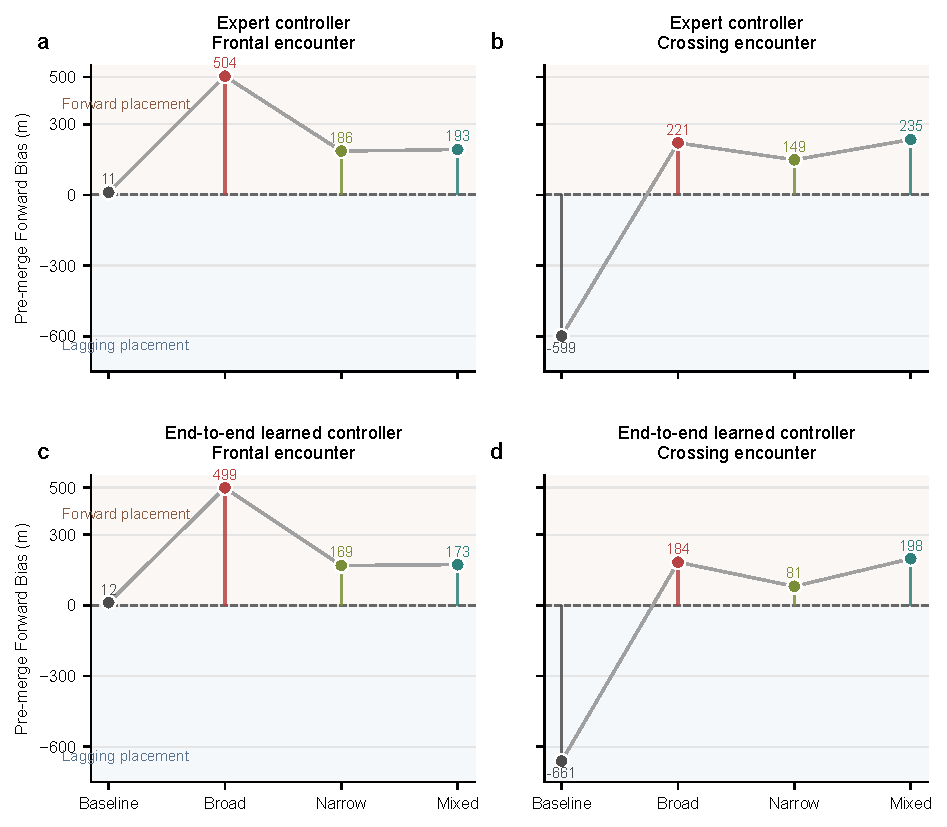
\includegraphics[width=\linewidth]{figures/figure3_forward_bias.pdf}
\caption{Pre-merge Forward Bias across interface variants. Each point shows the mean over the 10 pilot episodes for one interface variant. Broad global scaling drives all cells toward strongly positive forward placement, whereas the narrow and mixed variants reveal task-conditioned trade-offs. Positive values indicate forward placement of the virtual point in the counterpart-velocity frame, and negative values indicate lagging placement.}
\label{fig:forward_bias}
\end{figure}

\begin{figure}[H]
\centering
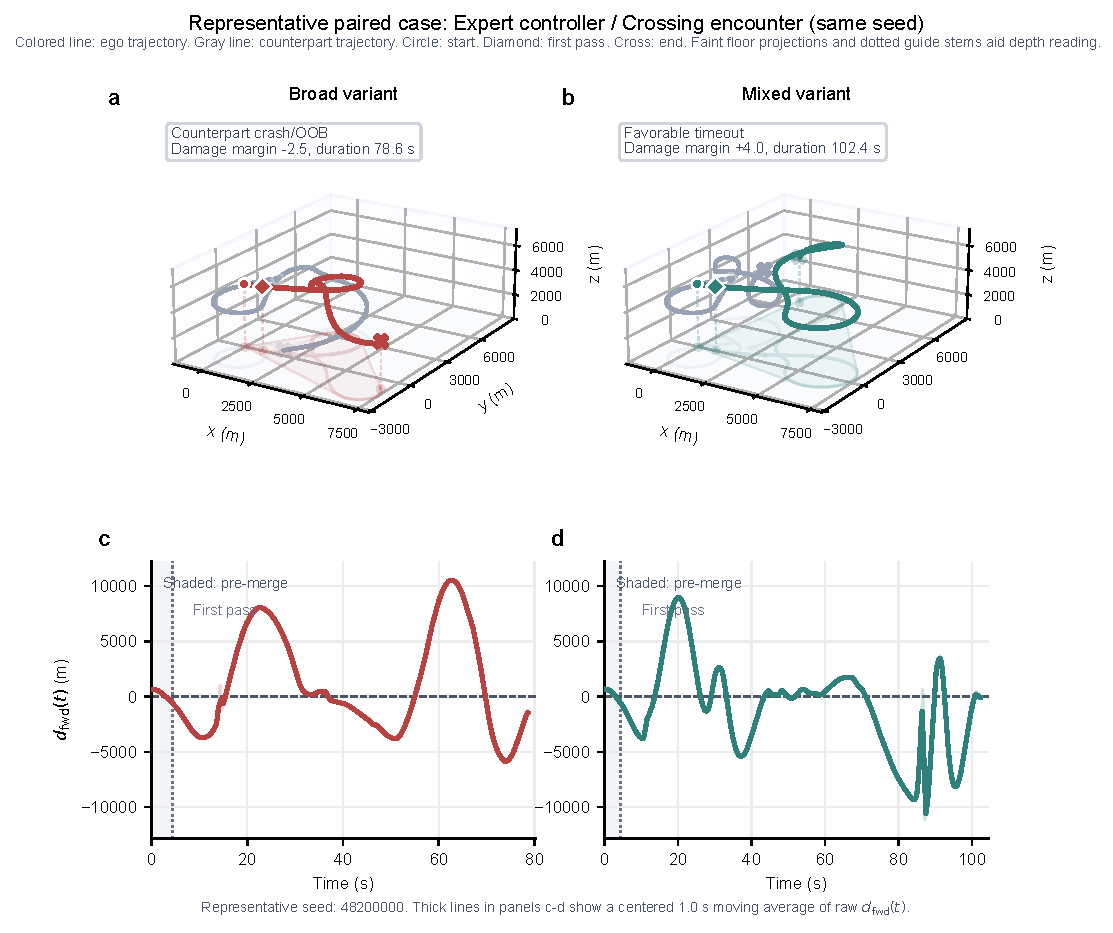
\includegraphics[width=\linewidth]{figures/figure4_representative_case.pdf}
\caption{Representative paired crossing-encounter case under the expert controller. Both columns use the same pilot seed. The upper panels show three-dimensional trajectories of the controlled UAV and the counterpart, with faint floor projections and guide stems included to aid depth perception. The broad variant reaches a favourable recorded outcome only because the counterpart leaves the admissible region despite a negative damage margin, whereas the mixed variant maintains a longer bounded interaction and finishes with a favourable timeout and a positive damage margin. The lower panels show the instantaneous Forward Bias trace $d_{\mathrm{fwd}}(t)$; the shaded interval marks the pre-merge phase and the dotted line marks first pass.}
\label{fig:representative_case}
\end{figure}

\begin{figure}[H]
\centering
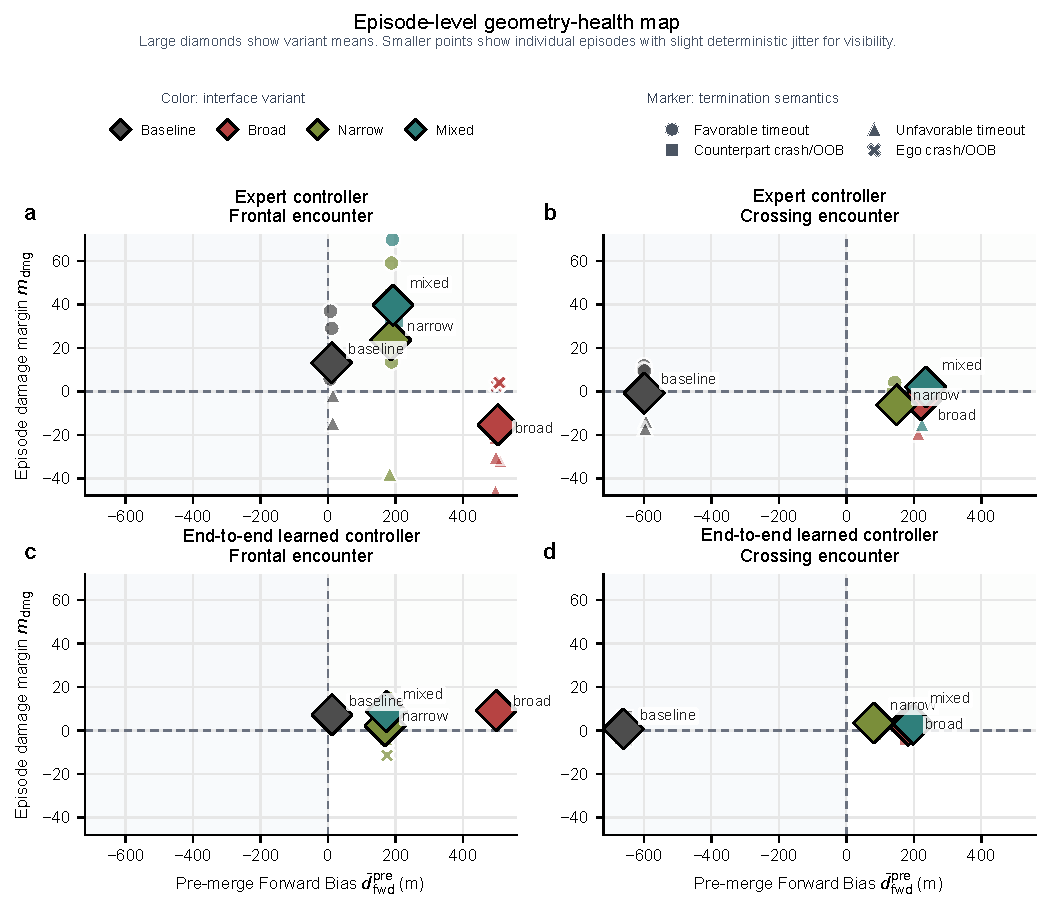
\includegraphics[width=\linewidth]{figures/figure5_geometry_health_map.pdf}
\caption{Episode-level geometry-health map across the 10 pilot episodes per interface variant. Each small point represents one episode, with slight deterministic jitter applied only for visibility; large diamonds show variant means. Horizontal position gives pre-merge Forward Bias and vertical position gives episode damage margin. Color encodes interface variant and marker shape encodes termination semantics. The expert frontal panel shows broad overreach as a far-right, negative-margin regime, whereas the expert crossing and end-to-end frontal panels show why Forward Bias alone is not sufficient: variants with similar forward-bias ranges can still separate by damage exchange and termination mode.}
\label{fig:geometry_health_map}
\end{figure}

\begin{table*}[t]
\centering
\caption{Summary of main results across four interface variants, two encounter classes, and two counterpart-controller settings. Win rate ($r_{\mathrm{fav}}$), damage margin ($m_{\mathrm{dmg}}$), pre-merge Forward Bias ($\bar{d}_{\mathrm{fwd}}^{\mathrm{pre}}$), and ego crash count are reported for each cell. Within each controller--encounter pair, the highest favourable outcome rate, the highest damage margin, and the lowest ego crash count are highlighted in \textbf{bold}; pre-merge Forward Bias is reported without bold ranking because it is interpreted as a geometry-health signal rather than as a monotonic objective.}
\label{tab:main_results}
\begin{tabular}{@{}llccccc@{}}
\toprule
Controller & Encounter & Variant & $r_{\mathrm{fav}}$ & $m_{\mathrm{dmg}}$ & $\bar{d}_{\mathrm{fwd}}^{\mathrm{pre}}$ (m) & Ego crashes \\
\midrule
Expert & Frontal & Baseline & 0.60 & 13.15 & 10.84 & 2 \\
& & Broad & 0.00 & $-15.40$ & 503.65 & 4 \\
& & Narrow & 0.90 & 23.70 & 185.92 & \textbf{0} \\
& & Mixed & \textbf{1.00} & \textbf{39.65} & 192.51 & \textbf{0} \\
\cmidrule{2-7}
& Crossing & Baseline & 0.30 & $-0.80$ & $-598.92$ & 1 \\
& & Broad & \textbf{0.90} & $-3.85$ & 220.69 & \textbf{0} \\
& & Narrow & 0.20 & $-6.20$ & 148.90 & 2 \\
& & Mixed & \textbf{0.90} & \textbf{2.05} & 234.84 & \textbf{0} \\
\midrule
End-to-end & Frontal & Baseline & \textbf{0.90} & 7.30 & 11.94 & \textbf{1} \\
& & Broad & \textbf{0.90} & \textbf{9.15} & 498.76 & \textbf{1} \\
& & Narrow & 0.20 & 2.25 & 169.34 & 7 \\
& & Mixed & \textbf{0.90} & 8.70 & 173.11 & \textbf{1} \\
\cmidrule{2-7}
& Crossing & Baseline & \textbf{1.00} & 0.75 & $-660.51$ & \textbf{0} \\
& & Broad & \textbf{1.00} & 2.50 & 183.58 & \textbf{0} \\
& & Narrow & \textbf{1.00} & \textbf{3.45} & 80.79 & \textbf{0} \\
& & Mixed & \textbf{1.00} & 2.90 & 198.20 & \textbf{0} \\
\bottomrule
\end{tabular}
\end{table*}

\section{Discussion}

\subsection{From Point Tracking to an Auditable Guidance Interface}

The main contribution of this study is a shift in what the virtual-point action layer means. Under the baseline formulation, the policy emits Cartesian offsets whose geometric intent must be inferred indirectly from the resulting trajectory. Under the geometry-basis formulation, the same three-dimensional action head becomes a structured interface whose coefficients have explicit longitudinal, lateral, and vertical meanings. This does not make the policy fully transparent, but it does move an important part of the decision pathway from an implicit representation into an inspectable one. For a guidance system that may later require trust-oriented validation, that is a meaningful architectural change \cite{glanois2024,paterson2025}.

The empirical evidence shows that this semantic shift is not merely descriptive. Across the broad, narrow, and mixed variants, changing the action interpretation and its associated extent parameters produced large, measurable differences in Forward Bias, termination mix, and damage exchange while leaving the policy dimensionality and downstream guidance stack unchanged. This makes the geometry-basis layer a useful attribution boundary: when behaviour changes, the analyst can relate that change to interpretable coefficients, extent choices, and geometry-health diagnostics rather than treating the policy as a monolithic black box. In that sense, the proposed interface serves as a white-box layer between the learned controller and the established guidance machinery.

\subsection{Why Universal Amplitude Scaling Fails}

The broad and narrow variants together explain why a single global amplitude rule is not an adequate design principle for this interface family. The broad variant showed that large extents can push all comparison cells toward strongly positive Forward Bias, sometimes with severe degradation in favourable outcomes and sometimes with seemingly acceptable scalar performance that is actually driven by counterpart failure modes. The narrow variant moved those values downward and repaired the expert-controller frontal encounter, but the same shrinkage simultaneously damaged the end-to-end frontal encounter and the expert-controller crossing encounter. The evidence therefore rules out a simple interpretation in which ``more reach'' is always harmful or ``less reach'' is always safer.

The coefficient summaries clarify the mechanism behind this failure. Across variants, the learned controller continued to prefer similar lead-lag and climb-descent directions, which means that the main source of change was the metric realisation of those preferences rather than a complete reorganisation of action tendencies. A global scaling factor is too blunt because it assumes that one conversion from coefficient space to world geometry can satisfy all encounter classes and counterpart-controller responses. The present results show that this assumption is false even within the limited scope of two encounter classes and two counterpart-controller classes.

\subsection{Task-Conditioned Interface Design as the Proper Interpretation}

The mixed variant suggests a more useful interpretation of the design problem. It preserved the narrow frontal-encounter extents that repaired the most obvious overreach case, while restoring the crossing-encounter extents needed to recover lost geometric reach. The resulting behaviour was not universally optimal, but it was the first variant in the current family to improve both expert-controller cells without reintroducing the narrow variant's end-to-end frontal collapse. This is why the mixed configuration is better understood as evidence for task-conditioned interface design than as proof that one final setting has solved the entire problem.

This interpretation matters for how the paper's contribution should be read. The present study does not claim that a single universally stable geometry-basis policy has been identified. Instead, it shows that a small, interpretable family of interface variants can expose structured trade-offs that would be difficult to understand under raw Cartesian action semantics alone. For a methods-oriented article, that is already a substantial result: the interface semantics, telemetry, and diagnostics make it possible to compare guidance designs on the basis of geometry health and termination structure, not only on headline outcome rate.

\subsection{Implications for Trustworthy Autonomous Guidance}

These findings have practical implications for trustworthy autonomous guidance design. First, they suggest that interpretable action semantics can be introduced without expanding the action head or rewriting the downstream guidance stack, which lowers the integration cost for existing virtual-point pipelines. Second, they show that step-level telemetry and aggregate diagnostics such as Forward Bias can function as early-warning indicators when a learned controller begins to realise an unstable geometry. Third, they demonstrate that separated termination semantics are essential for responsible evaluation because favourable outcome rate alone can hide whether improvements arise from healthier interaction structure or from counterpart failure modes.

More broadly, the study supports a view of guidance interfaces as assurance-relevant evidence surfaces rather than as passive wiring around a learned policy. If an autonomy stack is to be trusted, developers need access to quantities that remain stable enough to compare across variants and meaningful enough to explain failures when aggregate performance shifts \cite{paterson2025}. The geometry-basis layer does not solve that assurance problem on its own, but it makes the problem more tractable by exposing a compact set of semantically grounded variables and reproducible diagnostics. That is the central practical value of moving from virtual-point tracking toward an auditable geometry-shaping interface.

\section{Limitations and Responsible Use}

The present study has several limitations that should constrain its interpretation. First, the evaluation was conducted at pilot scale (10 seeds) rather than as a large held-out benchmark. Although the paired-seed design is reproducible, the statistical power is limited, and some of the observed differences may not persist under a larger formal campaign. Second, the scope was limited to two encounter classes and two counterpart-controller settings. Whether the task-conditioned design principle generalises to more diverse encounter geometries (for example, rear-quarter or beam approaches) remains to be tested. Third, the geometry-basis interface is a semantic reinterpretation rather than a new policy architecture; it cannot compensate for a poorly trained policy or an insufficient observation model. Fourth, the Forward Bias metric is an aggregate health indicator, not a standalone optimisation target. Using it as a direct reward signal could introduce unforeseen side effects. Accordingly, the numerical differences reported here should be read as pilot-scale design evidence and hypothesis-generating signals, not as definitive estimates of held-out generalisation.

In terms of responsible use, the geometry-basis interface and its telemetry are intended to support auditability and diagnostic analysis, not to provide an absolute safety guarantee. The separation of favourable outcome rate, damage margin, and termination categories is designed to prevent over-optimistic interpretation of aggregate metrics, but it does not replace the need for formal verification or domain-expert review. The present analysis is offered to improve transparency and evaluation discipline in autonomy research rather than to support operational decision-making. Any deployment of this interface in a real UAV system would require additional validation, including hardware-in-the-loop testing and independent safety assessment.

\section{Conclusion}

This paper has shown that a conventional three-dimensional virtual-point action head can be reinterpreted as a geometry-basis guidance interface whose coefficients directly modulate longitudinal, lateral, and vertical geometry components. The interface preserves the original policy network and action dimensionality while adding explicit semantic structure and diagnostic instrumentation, including a pre-merge Forward Bias metric that links action semantics to trajectory-level behaviour. Through a controlled pilot comparison of baseline, broad, narrow, and mixed variants across frontal and crossing close-range encounters, we found that the semantic reinterpretation produces large, measurable geometry shifts even when the policy backbone is unchanged. The pilot evidence further indicates that global amplitude scaling is too blunt for this task family: broad scaling destabilises some encounters, narrow scaling repairs one lane at the cost of regressions elsewhere, and a task-selective mixed design provided the strongest observed balance in the present comparison. These findings position virtual-point guidance not only as a tracking mechanism, but as an auditable geometry-shaping interface whose stability depends on task-conditioned design rather than universal parameter tuning.

\institutionalreview{Not applicable.}

\informedconsent{Not applicable.}

\dataavailability{The manuscript source files, figure-generation scripts, and source data used to generate Figures~1--5 are available in the project repository used to prepare this manuscript. Additional evaluation artifacts, configuration files, and episode-level logs are available from the corresponding authors upon reasonable request.}

\durcstatement{This study concerns auditable interface semantics and reproducible diagnostics for high-fidelity simulated UAV interaction. It does not report hardware deployment, field testing, or operational procedures. The work is presented to improve transparency, evaluation discipline, and responsible autonomy research; it is not intended as guidance for harmful or unlawful use.}

\acknowledgments{Generative-AI-assisted tooling was used during manuscript preparation for language revision, structural editing, and figure-code generation under direct author supervision. All technical claims, numerical values, and final wording were reviewed and approved by the authors.}

% Submission TODO: add author-contribution, funding, and conflict-of-interest
% statements after author confirmation rather than inferring them here.

\begin{thebibliography}{99}

\bibitem{choi2023}
J. Choi, H. M. Kim, H. J. Hwang, Y.-D. Kim, and C. O. Kim,
``Modular Reinforcement Learning for Autonomous UAV Flight Control,''
\emph{Drones}, vol. 7, no. 7, art. 418, 2023.
doi: 10.3390/drones7070418.

\bibitem{elmokadem2021}
T. Elmokadem and A. V. Savkin,
``Towards Fully Autonomous UAVs: A Survey,''
\emph{Sensors}, vol. 21, no. 18, art. 6223, 2021.
doi: 10.3390/s21186223.

\bibitem{glanois2024}
C. Glanois, P. Weng, M. Zimmer, D. Li, T. Yang, J. Hao, and W. Liu,
``A Survey on Interpretable Reinforcement Learning,''
\emph{Machine Learning}, vol. 113, pp. 5847--5890, 2024.
doi: 10.1007/s10994-024-06543-w.

\bibitem{park2007}
S. Park, J. Deyst, and J. P. How,
``Performance and Lyapunov Stability of a Nonlinear Path-Following Guidance Method,''
\emph{Journal of Guidance, Control, and Dynamics}, vol. 30, no. 6, pp. 1718--1728, 2007.
doi: 10.2514/1.28957.

\bibitem{paterson2025}
C. Paterson, R. D. Hawkins, C. Picardi, Y. Jia, R. Calinescu, and I. Habli,
``Safety Assurance of Machine Learning for Autonomous Systems,''
\emph{Reliability Engineering and System Safety}, vol. 264, art. 111311, 2025.
doi: 10.1016/j.ress.2025.111311.

\bibitem{quan2026}
S. Quan, S. Cao, C. Wang, and H. Yu,
``Autonomous Maneuvering Decision-Making Method for Unmanned Aerial Vehicle Based on Soft Actor-Critic Algorithm,''
\emph{Drones}, vol. 10, no. 1, art. 35, 2026.
doi: 10.3390/drones10010035.

\bibitem{ratnoo2015}
A. Ratnoo, S. Y. Hayoun, A. Granot, and T. Shima,
``Path Following Using Trajectory Shaping Guidance,''
\emph{Journal of Guidance, Control, and Dynamics}, vol. 38, no. 1, pp. 106--116, 2015.
doi: 10.2514/1.G000300.

\bibitem{lai2026aerospace}
Y. Lai, Y. Chen, Y. Yang, J. Jian, and Y. Liu,
``Hierarchical Decision-Making for UAV Close-Range Dynamic Tracking Using a Pursuit-Strategy Action Space,''
\emph{Aerospace}, vol. 13, no. 6, art. 508, 2026.
doi: 10.3390/aerospace13060508.

\bibitem{xu2022ast}
J. Xu, J. Zhang, L. Yang, and C. Liu,
``Autonomous Decision-Making for Dogfights Based on a Tactical Pursuit Point Approach,''
\emph{Aerospace Science and Technology}, vol. 129, art. 107857, 2022.
doi: 10.1016/j.ast.2022.107857.

\bibitem{schulman2017}
J. Schulman, F. Wolski, P. Dhariwal, A. Radford, and O. Klimov,
``Proximal Policy Optimization Algorithms,''
\emph{arXiv preprint arXiv:1707.06347}, 2017.

\bibitem{haarnoja2018}
T. Haarnoja, A. Zhou, P. Abbeel, and S. Levine,
``Soft Actor-Critic: Off-Policy Maximum Entropy Deep Reinforcement Learning with a Stochastic Actor,''
\emph{Proceedings of the 35th International Conference on Machine Learning (ICML)}, 2018, pp. 1861--1870.

\bibitem{kwak2025applsci}
N. J. Kwak, J. H. Lee, and S. Kim,
``The Evolution and Taxonomy of Deep Learning Models for Aircraft Trajectory Prediction: A Review of Performance and Future Directions,''
\emph{Applied Sciences}, vol. 15, no. 19, art. 10739, 2025.
doi: 10.3390/app151910739.

\bibitem{paleja2022}
R. Paleja, Y. Niu, A. Silva, C. Ritchie, S. Choi, and M. Gombolay,
``Learning Interpretable, High-Performing Policies for Autonomous Driving,''
\emph{Robotics: Science and Systems (RSS)}, 2022.

\bibitem{thomas2021}
D. G. Thomas, M. R. K. Reddy, and V. K. Chandrasekar,
``Interpretable UAV Collision Avoidance Using Deep Reinforcement Learning,''
\emph{arXiv preprint arXiv:2105.12254}, 2021.

\bibitem{wang2023aerospace}
L. Wang, J. Wang, H. Liu, and T. Yue,
``Decision-Making Strategies for Close-Range Air Combat Based on Reinforcement Learning with Variable-Scale Actions,''
\emph{Aerospace}, vol. 10, no. 5, art. 401, 2023.
doi: 10.3390/aerospace10050401.

\bibitem{chen2025aerospace}
C. Chen, T. Song, L. Mo, M. Lv, and D. Lin,
``Autonomous Dogfight Decision-Making for Air Combat Based on Reinforcement Learning with Automatic Opponent Sampling,''
\emph{Aerospace}, vol. 12, no. 3, art. 265, 2025.
doi: 10.3390/aerospace12030265.

\bibitem{zhu2024dt}
J. Zhu, M. Kuang, W. Zhou, H. Shi, J. Zhu, and X. Han,
``Mastering Air Combat Game with Deep Reinforcement Learning,''
\emph{Defence Technology}, vol. 34, pp. 295--312, 2024.
doi: 10.1016/j.dt.2023.08.019.

\bibitem{yang2020access}
Q. Yang, J. Zhang, G. Shi, J. Hu, and Y. Wu,
``Maneuver Decision of UAV in Short-Range Air Combat Based on Deep Reinforcement Learning,''
\emph{IEEE Access}, vol. 8, pp. 363--378, 2020.
doi: 10.1109/ACCESS.2019.2963172.

\bibitem{han2024smc}
H. Han and J. Cheng,
``Interpretable DRL-Based Maneuver Decision of UCAV Dogfight,''
in \emph{IEEE International Conference on Systems, Man, and Cybernetics (SMC)}, 2024, pp. 109--114.
doi: 10.1109/SMC.2024.10831270.

\bibitem{jing2024aerospace}
X. Jing, F. Cong, J. Huang, C. Tian, and Z. Su,
``Autonomous Maneuvering Decision-Making Algorithm for Unmanned Aerial Vehicles Based on Node Clustering and Deep Deterministic Policy Gradient,''
\emph{Aerospace}, vol. 11, no. 12, art. 1055, 2024.
doi: 10.3390/aerospace11121055.

\bibitem{fan2022machines}
Z. Fan, Y. Xu, Y. Kang, and D. Luo,
``Air Combat Maneuver Decision Method Based on A3C Deep Reinforcement Learning,''
\emph{Machines}, vol. 10, no. 11, art. 1033, 2022.
doi: 10.3390/machines10111033.

\bibitem{qi2023applsci}
W. Qi, J. Cheng, Y. Zhang, and H. Wang,
``Curved-Line Path-Following Control of Fixed-Wing Unmanned Aerial Vehicles Using a Robust Disturbance-Estimator-Based Predictive Control Approach,''
\emph{Applied Sciences}, vol. 13, no. 20, art. 11577, 2023.
doi: 10.3390/app132011577.

\bibitem{dubins1957}
L. E. Dubins,
``On Curves of Minimal Length with a Constraint on Average Curvature, and with Prescribed Initial and Terminal Positions and Tangents,''
\emph{American Mathematical Monthly}, vol. 64, no. 1, pp. 39--52, 1957.
doi: 10.1080/00029890.1957.11988969.

\bibitem{sujit2014}
P. B. Sujit, S. Saripalli, and J. B. Sousa,
``Unmanned Aerial Vehicle Path Following: A Survey and Analysis of Algorithms for Fixed-Wing Unmanned Aerial Vehicles,''
\emph{IEEE Control Systems}, vol. 34, no. 1, pp. 42--59, 2014.
doi: 10.1109/MCS.2013.2284950.

\bibitem{breivik2005}
M. Breivik and T. I. Fossen,
``Principles of Guidance-Based Path Following in 2D and 3D,''
in \emph{Proceedings of the 44th IEEE Conference on Decision and Control (CDC)}, 2005, pp. 627--634.

\bibitem{isaacs1965}
R. Isaacs,
\emph{Differential Games: A Mathematical Theory with Applications to Warfare and Pursuit, Control and Optimization}.
New York: Wiley, 1965.

\bibitem{zarchan2012}
P. Zarchan,
\emph{Tactical and Strategic Missile Guidance}, 6th ed.
Reston, VA: AIAA Progress in Aeronautics and Astronautics, 2012.

\bibitem{rhee2010}
I. Rhee and S. Park,
``A Study of the Pipelined Nonlinear Guidance for Path Following,''
\emph{Journal of the Korean Society for Aeronautical and Space Sciences}, vol. 38, no. 5, pp. 418--425, 2010.

\bibitem{mnih2015}
V. Mnih, K. Kavukcuoglu, D. Silver, A. Rusu, J. Veness, M. Bellemare, et al.,
``Human-Level Control Through Deep Reinforcement Learning,''
\emph{Nature}, vol. 518, pp. 529--533, 2015.
doi: 10.1038/nature14236.

\bibitem{gunning2019}
D. Gunning, M. Stefik, J. Choi, T. Miller, S. Stumpf, and G. Z. Yang,
``XAI---Explainable Artificial Intelligence,''
\emph{Science Robotics}, vol. 4, no. 37, eaay7120, 2019.
doi: 10.1126/scirobotics.aay7120.

\end{thebibliography}

\end{document}
